\documentclass[journal,12pt,twocolumn]{IEEEtran}

\usepackage{setspace}
\usepackage{gensymb}
\singlespacing
\usepackage[cmex10]{amsmath}

\usepackage{amsthm}

\usepackage{mathrsfs}
\usepackage{txfonts}
\usepackage{stfloats}
\usepackage{bm}
\usepackage{cite}
\usepackage{cases}
\usepackage{subfig}

\usepackage{longtable}
\usepackage{multirow}

\usepackage{enumitem}
\usepackage{mathtools}
\usepackage{steinmetz}
\usepackage{tikz}
\usepackage{circuitikz}
\usepackage{verbatim}
\usepackage{tfrupee}
\usepackage[breaklinks=true]{hyperref}
\usepackage{graphicx}
\usepackage{tkz-euclide}

\usetikzlibrary{calc,math}
\usepackage{listings}
    \usepackage{color}                                            %%
    \usepackage{array}                                            %%
    \usepackage{longtable}                                        %%
    \usepackage{calc}                                             %%
    \usepackage{multirow}                                         %%
    \usepackage{hhline}                                           %%
    \usepackage{ifthen}                                           %%
    \usepackage{lscape}     
\usepackage{multicol}
\usepackage{chngcntr}

\DeclareMathOperator*{\Res}{Res}

\renewcommand\thesection{\arabic{section}}
\renewcommand\thesubsection{\thesection.\arabic{subsection}}
\renewcommand\thesubsubsection{\thesubsection.\arabic{subsubsection}}

\renewcommand\thesectiondis{\arabic{section}}
\renewcommand\thesubsectiondis{\thesectiondis.\arabic{subsection}}
\renewcommand\thesubsubsectiondis{\thesubsectiondis.\arabic{subsubsection}}


\hyphenation{op-tical net-works semi-conduc-tor}
\def\inputGnumericTable{}                                 %%

\lstset{
%language=C,
frame=single, 
breaklines=true,
columns=fullflexible
}
\begin{document}


\newtheorem{theorem}{Theorem}[section]
\newtheorem{problem}{Problem}
\newtheorem{proposition}{Proposition}[section]
\newtheorem{lemma}{Lemma}[section]
\newtheorem{corollary}[theorem]{Corollary}
\newtheorem{example}{Example}[section]
\newtheorem{definition}[problem]{Definition}

\newcommand{\BEQA}{\begin{eqnarray}}
\newcommand{\EEQA}{\end{eqnarray}}
\newcommand{\define}{\stackrel{\triangle}{=}}
\bibliographystyle{IEEEtran}
\raggedbottom
\setlength{\parindent}{0pt}
\providecommand{\mbf}{\mathbf}
\providecommand{\pr}[1]{\ensuremath{\Pr\left(#1\right)}}
\providecommand{\qfunc}[1]{\ensuremath{Q\left(#1\right)}}
\providecommand{\sbrak}[1]{\ensuremath{{}\left[#1\right]}}
\providecommand{\lsbrak}[1]{\ensuremath{{}\left[#1\right.}}
\providecommand{\rsbrak}[1]{\ensuremath{{}\left.#1\right]}}
\providecommand{\brak}[1]{\ensuremath{\left(#1\right)}}
\providecommand{\lbrak}[1]{\ensuremath{\left(#1\right.}}
\providecommand{\rbrak}[1]{\ensuremath{\left.#1\right)}}
\providecommand{\cbrak}[1]{\ensuremath{\left\{#1\right\}}}
\providecommand{\lcbrak}[1]{\ensuremath{\left\{#1\right.}}
\providecommand{\rcbrak}[1]{\ensuremath{\left.#1\right\}}}
\theoremstyle{remark}
\newtheorem{rem}{Remark}
\newcommand{\sgn}{\mathop{\mathrm{sgn}}}
\providecommand{\abs}[1]{\left\vert#1\right\vert}
\providecommand{\res}[1]{\Res\displaylimits_{#1}} 
\providecommand{\norm}[1]{\left\lVert#1\right\rVert}
%\providecommand{\norm}[1]{\lVert#1\rVert}
\providecommand{\mtx}[1]{\mathbf{#1}}
\providecommand{\mean}[1]{E\left[ #1 \right]}
\providecommand{\fourier}{\overset{\mathcal{F}}{ \rightleftharpoons}}
%\providecommand{\hilbert}{\overset{\mathcal{H}}{ \rightleftharpoons}}
\providecommand{\system}{\overset{\mathcal{H}}{ \longleftrightarrow}}
\providecommand{\ztrans}{\overset{\mathcal{Z}}{ \rightleftharpoons}}
	%\newcommand{\solution}[2]{\textbf{Solution:}{#1}}
\newcommand{\solution}{\noindent \textbf{Solution: }}
\newcommand{\cosec}{\,\text{cosec}\,}
\providecommand{\dec}[2]{\ensuremath{\overset{#1}{\underset{#2}{\gtrless}}}}
\newcommand{\myvec}[1]{\ensuremath{\begin{pmatrix}#1\end{pmatrix}}}
\newcommand{\mydet}[1]{\ensuremath{}}
\numberwithin{equation}{subsection}

\makeatletter
\@addtoreset{figure}{problem}
\makeatother
\let\StandardTheFigure\thefigure
\let\vec\mathbf

\renewcommand{\thefigure}{\theproblem}

\def\putbox#1#2#3{\makebox[0in][l]{\makebox[#1][l]{}\raisebox{\baselineskip}[0in][0in]{\raisebox{#2}[0in][0in]{#3}}}}
     \def\rightbox#1{\makebox[0in][r]{#1}}
     \def\centbox#1{\makebox[0in]{#1}}
     \def\topbox#1{\raisebox{-\baselineskip}[0in][0in]{#1}}
     \def\midbox#1{\raisebox{-0.5\baselineskip}[0in][0in]{#1}}
\vspace{3cm}
\title{Gate Assignment 4}
\author{Tanmay Goyal - AI20BTECH11021}
\maketitle
\newpage
\bigskip
\renewcommand{\thefigure}{\theenumi}
\renewcommand{\thetable}{\theenumi}

Download all latex codes from 
\begin{lstlisting}
https://github.com/tanmaygoyal258/EE3900-Linear-Systems-and-Signal-processing/blob/main/GateAssignment4/main.tex
\end{lstlisting}
\section{Problem}
(EC-2001/Q.16) The Fourier Transform $G(\omega)$ of the signal $g(t)$ is given by 
\begin{align}
    G(\omega) = \frac{1}{\omega^2}(e^{j\omega} - j\omega e^{j\omega} - 1)
\end{align}
Using this information, find the Fourier Transforms of the signals $g_1(t)$, $g_2(t)$ and $g_3(t)$.
\begin{figure}[!ht]
\centering
 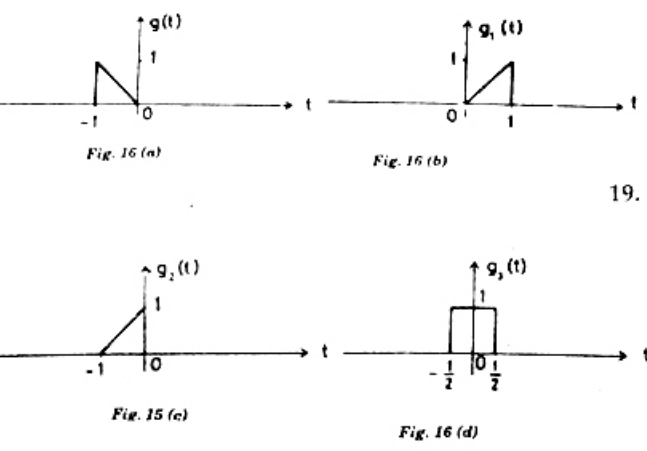
\includegraphics[width=\columnwidth]{Question.png}
\end{figure}
\section{Solution}
We replace $\omega$ by $2\pi f$.
Then, 
\begin{align}
    G(f) = \frac{1}{4\pi^2 f^2}(e^{2\pi jf} - 2\pi jf e^{2\pi jf} -1)
\end{align}\\

\begin{lemma}
If 
\begin{align}
    g(t) \fourier G(f)
\end{align}
then,
\begin{align}
    g(t \pm t_0) \fourier G(f)e^{\pm 2\pi j f t_0}
\end{align}
\label{shift}
\end{lemma} 

\begin{proof}
We know, 
\begin{align}
    G(f) = \int_{-\infty}^\infty g(t) e^{-2\pi j ft} \,dt
\end{align}
Let 
\begin{align}
    g(t + t_0) \fourier G'(f)
\end{align}
Then,
\begin{align}
    G'(f) = \int_{-\infty}^\infty g(t + t_0) e^{-2\pi j ft} \,dt
\end{align}
Substituting $t + t_0 = T$, we get:
\begin{align}
    G'(f) = \int_{-\infty}^\infty g(T) e^{-2\pi j f(T - t_0)} \,dT\\
     = \int_{-\infty}^\infty g(T) e^{-2\pi j fT} e^{2\pi j ft_0} \,dT\\
      =e^{2\pi j ft_0} \int_{-\infty}^\infty g(T) e^{2\pi j fT} \,dT\\
       = e^{-2\pi j ft_0}G(f)
\end{align}
Similarly, it can be proved:
 \begin{align}
     g(t - t_0) \fourier e^{-2\pi j ft_0}G(f)
 \end{align}
\end{proof}

\begin{lemma}
If 
\begin{align}
    g(t) \fourier G(f)
\end{align}
then,
\begin{align}
    g(\alpha t) \fourier \frac{1}{\abs{\alpha}}G\brak{\frac{f}{\alpha}}
\end{align}
\label{scale}
\end{lemma}
\begin{proof}
Consider $\alpha > 0$. Then, we know, 
\begin{align}
    G(f) = \int_{-\infty}^\infty g(t) e^{-2\pi j ft} \,dt
\end{align}
Let 
\begin{align}
    g(\alpha t) \fourier G'(f)
\end{align}
Then,
\begin{align}
    G'(f) = \int_{-\infty}^\infty g(\alpha t) e^{-2\pi j ft} \,dt
\end{align}
Making the substitution $T = \alpha t$, we get:
\begin{align}
     G'(f) = \frac{1}{\alpha}\int_{-\infty}^\infty g(T) e^{-2\pi j \frac{f T}{\alpha}} \,dT\\
     = \frac{1}{\alpha}G\brak{\frac{f}{\alpha}}
\end{align}
Similarly, it can be proved for $\alpha < 0$
\begin{align}
    g(\alpha t) \fourier \frac{-1}{\alpha}G\brak{\frac{-f}{\alpha}}
\end{align}
\end{proof}
\begin{lemma}
If 
\begin{align}
    g(t) \fourier G(f)
\end{align}
then,
\begin{align}
    g(- t) \fourier G(-f)
\end{align}
\label{reverse}
\end{lemma}
\begin{proof}
Put $\alpha = -1$ in \eqref{scale} to obtain the result.
\begin{align}
    g(-t) \fourier \frac{1}{\abs{-1}}G\brak{\frac{f}{-1}}\\
    g(-t) \fourier G(-f)
\end{align}
\end{proof}

Now, from the figure:
\begin{align}
    g(t) = 
    \begin{cases}
    -t & -1 \leq t \leq 0\\
    0 & otherwise
    \end{cases}\\
    g_1(t) = 
    \begin{cases}
    t & 0 \leq t \leq 1\\
    0 & otherwise
    \end{cases}\\
    g_2(t) = 
    \begin{cases}
    1+t & -1 \leq t \leq 0\\
    0 & otherwise
    \end{cases}\\
    g_3(t) = 
    \begin{cases}
    1 & -\frac{1}{2} \leq t \leq \frac{1}{2}\\
    0 & otherwise
    \end{cases}
\end{align}



Clearly, $g_1(t) = g(-t)$, and using \eqref{reverse}, we get:
\begin{align}
    G_1(f) = G(-f) = \frac{1}{4\pi^2f^2}(e^{-2\pi jf} + 2\pi jf e^{-2\pi jf} - 1)
\end{align}


Also, $g_2(t) = g(-t-1)$. Thus, from \eqref{shift} and \eqref{reverse}, we get:

\begin{align}
    g(t-1) \fourier e^{-2\pi jf}G(f)\\
    g(-t-1) \fourier e^{2\pi jf} G(-f)\\
    g_2(t) \fourier e^{2\pi jf}G(-f) \\
   g_2(t) \fourier \frac{1}{4\pi^2f^2}(1 + 2\pi jf  - e^{2\pi jf})\\
   \implies G_2(\omega) =  \frac{1}{4\pi^2f^2}(1 + 2\pi jf  - e^{2\pi jf})
\end{align}




Also, $g_3(t) = g\brak{t - \frac{1}{2}} + g\brak{-t - \frac{1}{2}}$. Thus, 
\begin{align}
    g\brak{t - \frac{1}{2}} \fourier e^{-j\pi f}G(f)\\
    g\brak{-t-\frac{1}{2}} \fourier e^{j\pi f}G(-f)\\
    g_3(t) \fourier e^{-j\pi f}G(f) + e^{j\pi f}G(-f)
    \end{align}
    \begin{multline}
    G_3(f)= \frac{e^{-j\pi f}}{4\pi^2f^2}\sbrak{e^{2\pi jf} - 2\pi jfe^{2\pi jf} - 1} + \\
    \frac{e^{j\pi f}}{4\pi^2f^2}\sbrak{ e^{-2\pi jf} + 2\pi jfe^{-2\pi jf} -1}\\
    \end{multline}
    \begin{align}
        G_3(f) = \frac{j}{2\pi f}\sbrak{e^{-\pi jf} - e^{\pi jf}}\\
        G_3(f) = \frac{\sin{\pi f}}{\pi f} = sinc(f)
    \end{align}
    where $sinc(t)$, the sampling function is defined as:
\begin{align}
    sinc(t) = 
    \begin{cases}
    1 & t = 0\\
    \frac{\sin(\pi t)}{\pi t} & otherwise
    \end{cases}
\end{align}
\begin{figure}[!ht]
\centering
 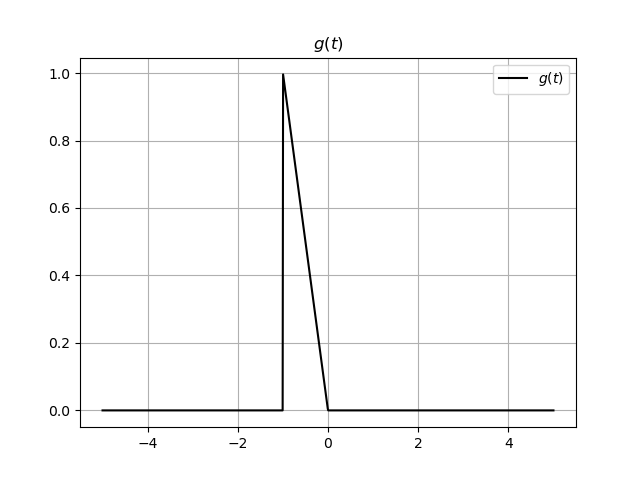
\includegraphics[width=\columnwidth]{graphs/g.png}
\end{figure}

\begin{figure}[!ht]
\centering
 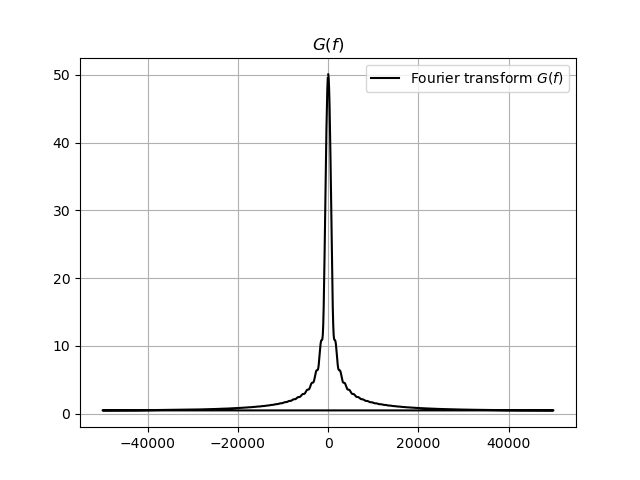
\includegraphics[width=\columnwidth]{graphs/fourier_g.png}
\end{figure}
    
\begin{figure}[!ht]
\centering
 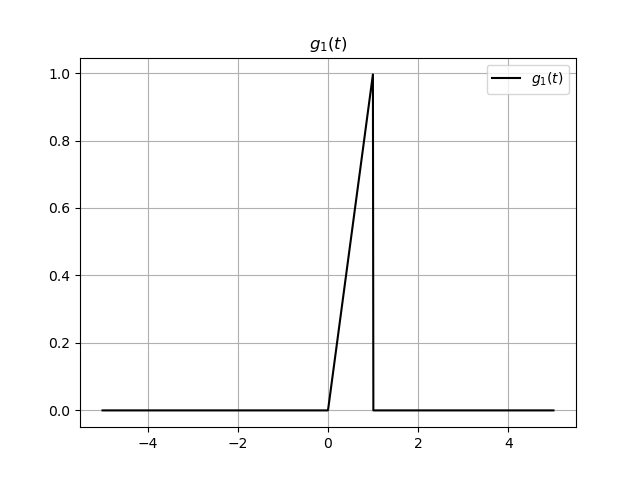
\includegraphics[width=\columnwidth]{graphs/g1.png}
\end{figure}

\begin{figure}[!ht]
\centering
 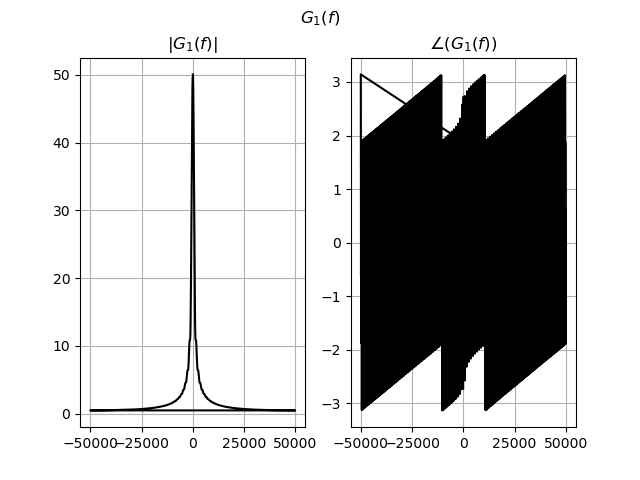
\includegraphics[width=\columnwidth]{graphs/fourier_g1.png}
\end{figure}

\begin{figure}[!ht]
\centering
 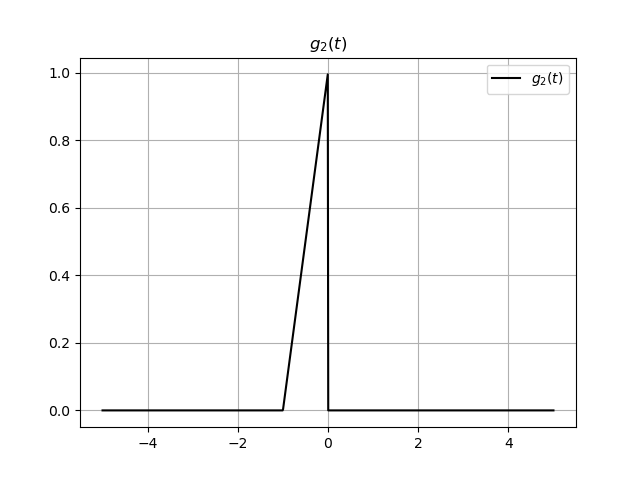
\includegraphics[width=\columnwidth]{graphs/g2.png}
\end{figure}

\begin{figure}[!ht]
\centering
 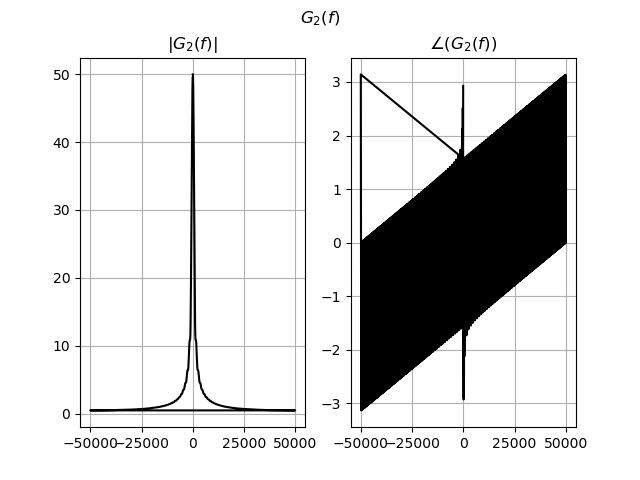
\includegraphics[width=\columnwidth]{graphs/fourier_g2.png}
\end{figure}    
    
    
\begin{figure}[!ht]
\centering
 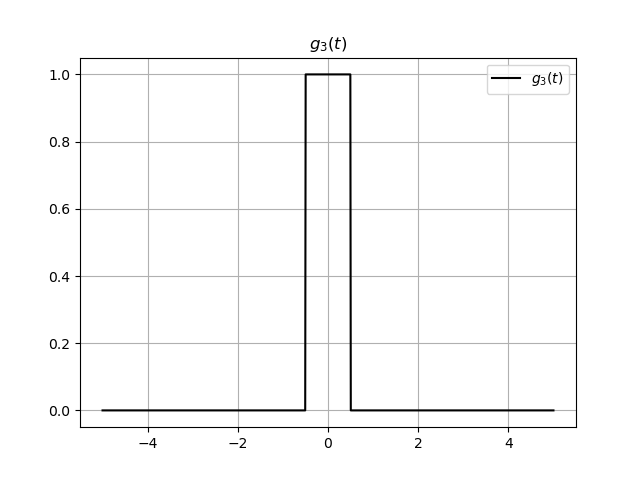
\includegraphics[width=\columnwidth]{graphs/g3.png}
\end{figure}

\begin{figure}[!ht]
\centering
 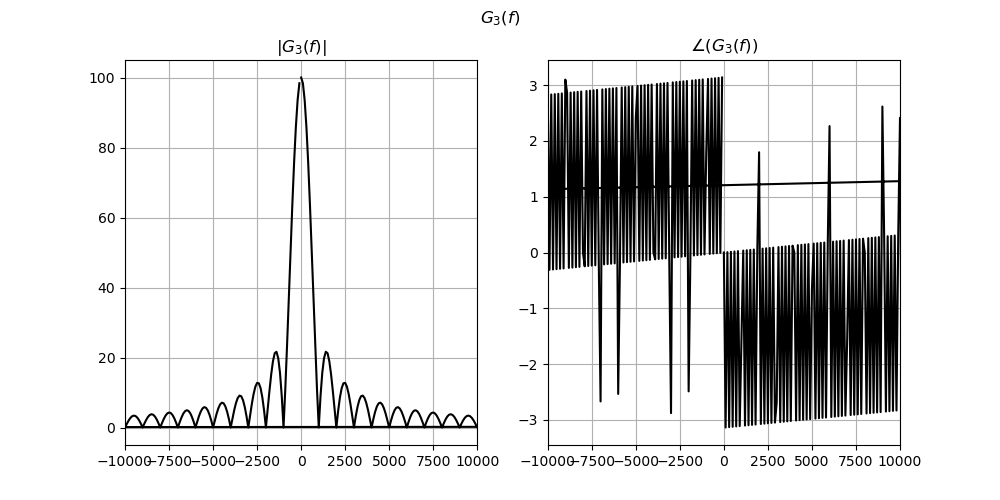
\includegraphics[width=\columnwidth]{graphs/fourier_g3.png}
\end{figure}
    
    
\end{document}
